\documentclass{article}

%------------------------------------------------------------------------------
%Packages
\usepackage{comment}
%\usepackage[francais]{babel}
\usepackage[latin1]{inputenc}
\usepackage[T1]{fontenc}
\usepackage{graphicx}

%------------------------------------------------------------------------------

\title{Plee the Bear - Graphism \\--- English version ---}
\author{Julien Jorge}
\date{\today}

\begin{document}

%------------------------------------------------------------------------------

\maketitle
\begin{abstract}
This document presents how the game deals with graphism and try to
explain which level of visual quality we want to reach. We will do a
fast presentation of the levels' structure, then we'll give some
details about the restrictions on the sprites and, finally, we'll give
some rules on how to draw good pictures.
\end{abstract}

\tableofcontents
\newpage

%------------------------------------------------------------------------------
\section{Level structure}
The levels are made of several layers (see
fig.~\ref{fig-layers-separated}). From the foreground to the
background, we have :
\begin{itemize}
\item one status layer, with scores, remaining lives, etc.
\item one ``bubbles'' layer, that show also the positions of the
      players that are out of the screen,
\item zero or more decoration layers, with sprites and animations,
\item one action layer, where players and enemies are,
\item zero ore more decoration layers.
\end{itemize}

The player's view is represented by a camera. We calculate the
current view with an orthogonal projection of the layers' content
through the camera box (see fig.~\ref{fig-layers-result}). We use the
action level as reference ; its size is exactly the size of the
world. Smallest layers will scroll slower, while biggest layers will
scroll faster. For example, a layer having half of the size of the
action layer on each axe will scroll two times slower.

\begin{figure}
 \begin{center}
  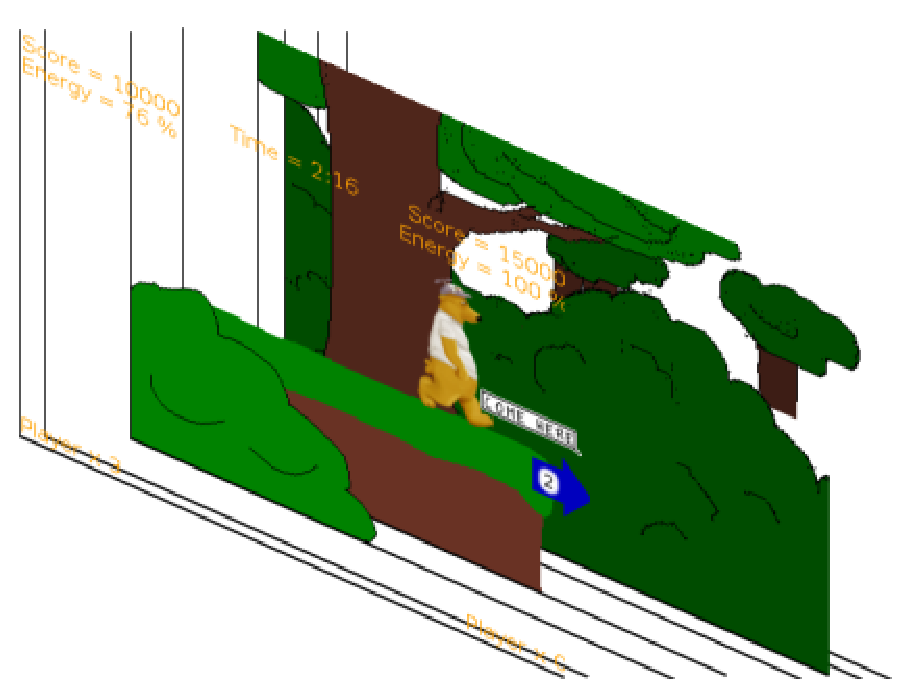
\includegraphics[width=9cm]{pictures/layers-separated}
  \caption{The different layers}
  \label{fig-layers-separated}
  \end{center}
\end{figure}

\begin{figure}
 \begin{center}
  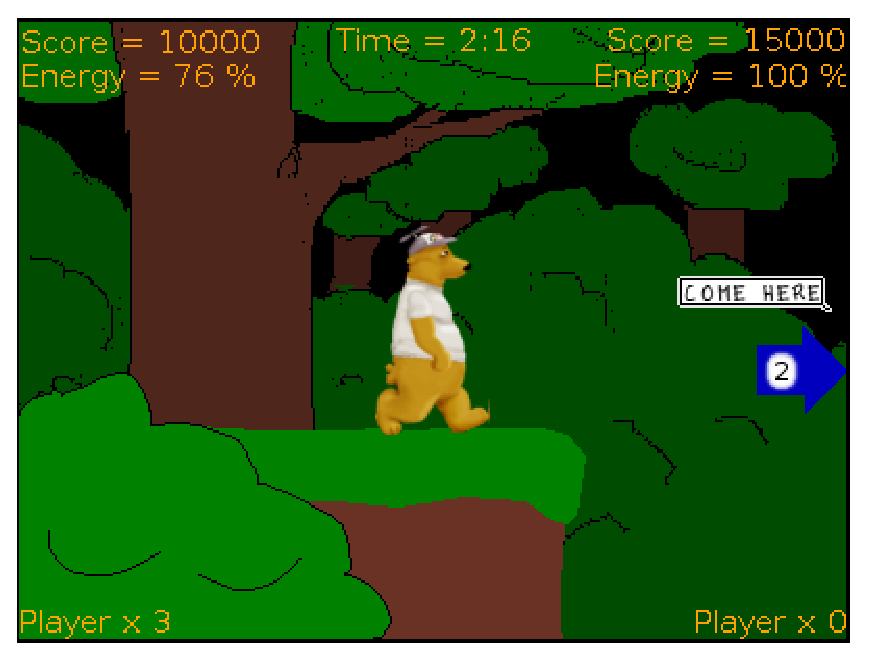
\includegraphics[width=9cm]{pictures/layers-result}
  \caption{The resulting view}
  \label{fig-layers-result}
 \end{center}
\end{figure}

\section{Sprites restrictions}
To give an idea of the scale of the sprites, the height of the player
is one third of the screen's height. Most of the time, he will be
placed in the middle of the screen.

The game doesn't do pixel-perfect collisions. Items are considered as
rectangles, they are in collision if their rectangles intersect. For
example, if your sprite is a line of 14 pixels with an angle of 45
degrees, it will be considered as a square box of 10 $\times$ 10
pixels. If two of those boxes intersect in only one pixel, there will
be a collision ; even if the lines seem to be far from each other. We
allow the boxes to have a size different of the size of the sprite, so
we can make some compromises.

Take the green circle of the figure~\ref{fig-bounding-box} as
example. Each box between the red squares is candidate for the
sprite's box. We will probably choose the intermediate box.  Although
the objects are reduced to rectangles, try to do pictures with
curves. The levels must not look like a set of square pieces put side
by side.

\begin{figure}
\begin{center}
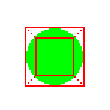
\includegraphics{pictures/bounding-box}
\caption{Bounding boxes for a circle}
\label{fig-bounding-box}
\end{center}
\end{figure}

\section{How to draw good pictures}

The game will looks like a carefully drawed picture ; something
between the flat drawing made by a child and the cold image that
can make a 3D-modelling software. You must think ``(beautiful) comic
strip'' :
\begin{itemize}
\item pictures must look ``hand-made'',
\item we should never see two times the same decoration sprite on a screen,
\item pictures must have as many details as possible.
\end{itemize}

\begin{figure}
   \begin{minipage}[c]{.46\linewidth}
     \begin{center}
      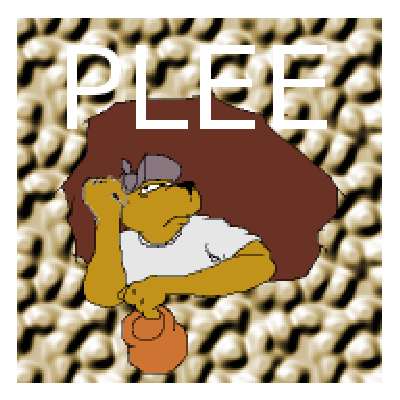
\includegraphics[width=5.5cm]{pictures/bad}
      \caption{Bad drawing}
      \label{fig-bad}
     \end{center}
   \end{minipage} \hfill
   \begin{minipage}[c]{.46\linewidth}
     \begin{center}
      
\includegraphics[width=5.5cm]{pictures/good}
      \caption{Good drawing}
      \label{fig-good}
     \end{center}
   \end{minipage}
\end{figure}

Let's take figures \ref{fig-bad} and \ref{fig-good} as examples. For
the first one, even if one can see and understand that Plee's is here,
with a honey pot in his hand, no one would want to look at this
picture more than one second. Even though the second picture is more
detailed, one would want to find all details, from the small nails to
the paint marks on Plee's arms.

Avoid repetitive textures and avoid any pictures provided with you
image manipulation software. The player must think ``Wow ! What a
beautiful and unique screen !'', not ``Hey ! They take that in
photoshop !''.

The final rule will be : ``if it's enough for you, try to do better''.

\end{document}
